\documentclass{article}%
\usepackage[T1]{fontenc}%
\usepackage[utf8]{inputenc}%
\usepackage{lmodern}%
\usepackage{textcomp}%
\usepackage{lastpage}%
\usepackage{authblk}%
\usepackage{graphicx}%
%
\title{Mannheimia haemolytica Leukotoxin Activates a Nonreceptor Tyrosine Kinase Signaling Cascade in Bovine Leukocytes, Which Induces Biological Effects}%
\author{Susan Cooper}%
\affil{State Key Laboratory of Cancer Biology and Xijing Hospital of Digestive Diseases, The Fourth Military Medical University, Xian, Shaanxi, People's Republic of China}%
\date{01{-}01{-}2011}%
%
\begin{document}%
\normalsize%
\maketitle%
\section{Abstract}%
\label{sec:Abstract}%
Our immune system works to protect us against the harmful effects of inflammation, particularly acute lung injury. As a result, proteins called PIAS1 surface to our peripheral blood to defend against neutropenia the symptoms that can lead to acute lung injury and death.\newline%
As the pressure within our body mounts from developing blood vessels, the PIAS1 protein rapidly begins releasing many of its potential carcinogens. Working against the fast{-}growing proteins, this naturally occurring body protein produces a lot of other toxic chemicals. This rapid release of PIAS1 and other "mad chemical molecules" is known as upregulation.\newline%
Levels of PIAS1 increase in the blood, rising to life{-}threatening levels. Clinical inflammation in the lungs increases the blood levels of this potentially lethal carcinogen and disease{-}causing toxin by nearly 1,000 percent.\newline%
Proteins carry the long{-}term messages to our cells to protect them from other harmful chemicals and human infections. However, these messages are also produced by PIAS1, and many drugs use the PIAS1 signaling molecule as an anti{-}inflammatory agent. In some people, these drugs alter PIAS1 production. In healthy individuals, the messages remain intact, while in illness they are disrupted.\newline%
However, in patients with severe acute pancreatitis, this time the message is compromised. An excess of PIAS1 accumulates in the livers of patients with severe acute pancreatitis, leaving them with chronic low blood levels of a deadly tumor{-}inducing substance.\newline%
A chemical in the body called tau{-}au represents the first line of defense against cancer, inflammation, and hepatitis. Humans to humans, tau{-}au binds to PIAS1, shutting down the PIAS1 process. When this process is disrupted, the pTO+ cell loses its ability to repress the PIAS1 signaling, which causes the tumor{-}forming protein to enter the blood stream, clogging arterial drainage lines, causing systemic infections, or even lethal cancers.

%
\subsection{Image Analysis}%
\label{subsec:ImageAnalysis}%


\begin{figure}[h!]%
\centering%
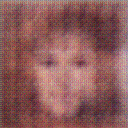
\includegraphics[width=150px]{500_fake_images/samples_5_443.png}%
\caption{A Cat Is Standing In Front Of A Mirror}%
\end{figure}

%
\end{document}